%!TEX root = ../main.tex
%=========================================================

\section{Placement of advertisements}
\label{sec:placement}

In the following, we detail the distribution of advertisements in the network and discuss the process of searching for, and establishing application-specific connections.
We start by discussing related challenges and explaining the data structures used by \sysname. 

\subsection{Challenges}

% \er{this straw man argument is a bit longish and a good candidate for fat trimming}

A first challenge in designing a robust service discovery mechanisms is to decide on the placement of advertisements (ads).
In other words, the mechanism must decide which registrars in the network should be responsible for storing ads for each service.

A first possibility would be to deterministically choose a group of nodes based on the service itself, using DHT lookups.
Such a solution makes it \emph{efficient} to place and retrieve ads, as both advertisers and discoverers know how to reach registrars within a logarithmic amount of steps.
Unfortunately, such an approach causes \emph{unequal} load distribution across registrars, especially when the popularity of services varies significantly.
Registrars storing popular services (\ie DHT nodes that are the closest to the hash of the popular services) would, indeed, receive a large portion of the registration requests in the network. 
Finally, this solution is \emph{not secure}, as an attacker could generate and strategically place its Sybil identities, and take control over all the traffic related to a single service. 

Alternatively, advertisers could place their ads on random registrars across the entire network. 
This approach, as \discv, is \emph{secure} and difficult to attack as an attacker would need to take control over the entire network to control a single service.
Furthermore, random placement is \emph{fair} and achieves good load balance across registrars regardless of the service popularity distribution.
However, and similarly again to \discv, random placement is not \emph{efficient}, as it makes it difficult for discoverers to find placed ads, especially for unpopular services. 

\sysname implements an alternative method of placing ads, that combines both the deterministic and pseudo-random approaches.
Advertisers start the registration process from nodes located far away from the service hash, and traverse the DHT towards nodes close to the service hash.
On their way, advertisers place ads on encountered registrars.
% This way, the closer to the service hash, the higher number of ads placed.
This way, as a registration process gets closer to the service hash, the higher the density of ads gets.
The discoverers mimic the process and ask encountered registrars for service-specific ads.
The lookup process stops when enough ads are found.

\subsection{Data structures}
\label{sec:struct}

\sysname uses two types of tables to handle registrations and lookups for service, the \emph{advertise} and \emph{search} tables.
Similarly to the Kademlia routing table, both tables are organized as a collection of \emph{buckets} $B(s) = \{b_0(s), b_1(s),..., b_m(s)\}$ but are centered around $s$ rather than the node ID.

The structure of these tables is similar but their use and lifecycles differ. 

%\para{Common tables structure}

%Buckets contain peers sharing a common prefix, and can be sorted by these prefixes (\eg, peers with ID starting with 0, 1, 2, and so on).
%Unlike the Kademlia routing table, however, advertise and search tables are centered on a target service ID rather than current node's ID, and prefixes represent different distances from this service ID.

\para{Advertise Table}
An advertiser maintains an \emph{advertise table} for each of the services it belongs to and advertises.
These tables exist for the whole duration of the participation to the corresponding service.
The table keeps track of ongoing registration attempts with different registrars.
Each bucket aims to contain \emph{at least} $K_\textit{register}$ potential registrars (\Cref{fig:advertise_table}).
Peers above the number of $K_\textit{register}$ are kept as backup peers.

\begin{figure}
    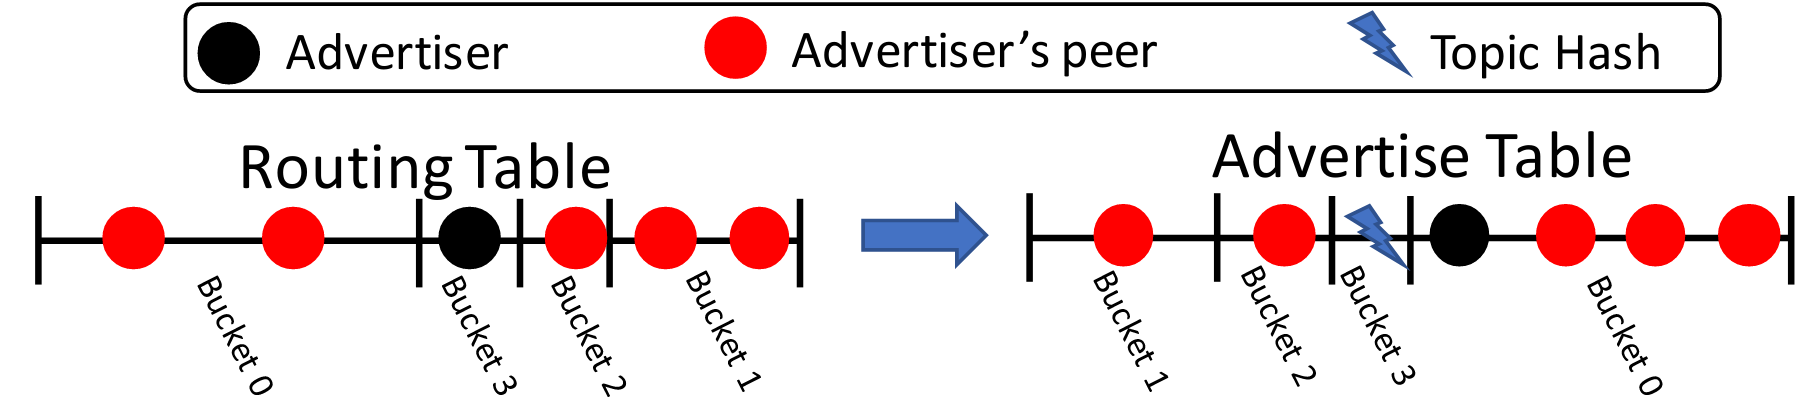
\includegraphics[width=0.45\textwidth]{img/tables}
    \vspace{-0.05in}
    \caption{Creation of an advertise table from a routing table.} %\mk{To be reworked and make it consistent with other figures. E.g., we shouldn't use a circle to represent the hash space. We can maybe also try to illustrate here the mechanism of placing a fixed amount of ads in each bucket.}}
    \label{fig:advertise_table}
    \vspace{-0.15in}
\end{figure}

\para{Search Table}
A specific search table is created for every new service discovery request.
This table is used to discover a number of ads through an iterative and parallel exploration process, after which the table is discarded.

\para{Construction and update of the tables}
Both tables are bootstrapped upon their creation (\ie, joining a new application for an advertise table and initiating a new discovery process for a search table) using entries from the local node routing table, for a specific service ID.
As the routing table is centered on the peer ID and not on this service ID, the density of peers around the latter might be low or even null, particularly when two IDs are distant in the key space.
The buckets are filled opportunistically while interacting with peers during the advertisement/lookup process.
There is, therefore, no specific DHT lookup for filling in the entries of these tables.

Malicious peers can however return large numbers of malicious nodes attempting to poison the routing process. To limit this risk, a local node $n_i$ communicating with peer $n_j$ in bucket $b_k(s)$ asks $n_j$ to return a single peer per bucket from $n_j$'s routing table for all buckets $b_l \:|\: l \geq k$. For instance, when communicating with a peer in bucket $b_{5}(s)$, $n_i$ only accepts a single candidate peer per buckets $b_5(s)$, $b_6(s)$, $b_7(s)$ and so on. Contacting nodes in buckets of increasing prefix length divides the search space by a constant factor, and allows learning new peers from more densely-populated routing tables towards the destination. The procedure mitigates the risk of having malicious peers polluting the table while still learning rare peers in buckets close to $s$. 


\subsection{Distributing ads across registrars}
\label{sec:registration_multi}


\Cref{alg:advertise} presents the advertisement procedure. The objective of the ad placement process is to continuously maintain up to $K_\textit{register}$ active (\ie, unexpired) registrations or ongoing registration attempts in every bucket of that table. 


An advertiser first creates a service-specific advertise table as detailed above.
Buckets located close to the service hash cover less hash space than buckets located further away and, in turn, contain fewer than $K_\textit{register}$ potential registrars; in this case, an attempt of registering an ad is made with all of them.

Placing a fixed amount of ads per bucket make registrars close to a service hash more likely to receive registrations for that specific service. 
Increasing $K_\textit{register}$ makes the advertiser easier to find at the cost of increased communication and storage costs.

The advertiser keeps track of pending or completed attempts to perform registrations in every bucket.
Registration may be unsuccessful if the selected registrar is down or refuses to store the ad.
In this case, the corresponding peer is removed from the bucket and a backup peer is selected as a replacement if one is available.\mk{Not shown in the alg at the moment but it seems like an implementation detail.}
A successful registration follows an admission procedure that we will detail in \Cref{sec:admission} and places an ad on an advertiser for a fixed amount of time $E$.

\begin{algorithm}[]%
    \caption{%
        Advertisement algorithm run by advertisers.
    }%
    \label{alg:advertise}%
    \begin{algorithmic}[1]%
         \footnotesize
        \State $\algvar{ongoing} \gets  \textsc{Map}\left \langle bucket;\textsc{list}\langle registrars \rangle \right \rangle$
        \State $B(s) \gets B(\algvar{self.id})$
        \item[]
        \Procedure{Advertise}{s}
            %\State $\algvar{regTable.initFromRoutingTables()}$
            \For{$i$ in $0, 1,..., m$}
                \If{$\algvar{ongoing[i].size} < K_{register}$}
                    \State $\algvar{registrar} \gets b_i(s)\algvar{.getRandomNode()}$
                    \State $\algvar{ongoing[i].add}(\algvar{registrar})$
                                   
                    \State $\algvar{ad.service} \gets s$
                    \State $\algvar{ad.ip} \gets \algvar{self.ip}$

                    \State $\algvar{async}(\Call{AdvertiseSingle}{\algvar{registrar}, \algvar{ad}, i})$
                \EndIf
            \EndFor
        \EndProcedure
        \item[]
        \Procedure{AdvertiseSingle}{\algvar{registrar}, \algvar{ad}, $i$}
            \While{True}
                \State $\algvar{response} \gets \algvar{registrar.Register(ad)}$
                \State $B(s)\algvar{.add}(\algvar{response.neighbors})$
                \If{$\algvar{response.status} = \algvar{Confirmed}$}
                    \State $\Call{sleep}{E}$
                    \State $\algvar{ongoing[i].remove}(\algvar{registrar})$
                    \State $\Return$
                \ElsIf{$\algvar{response.status} = \algvar{Wait}$}
                    \State $\Call{sleep}{\algvar{response.ticket.wait\_for}}$
                    \State $\algvar{ad.ticket} \gets \algvar{response.ticket}$
                \EndIf
            \EndWhile

        \EndProcedure
    \end{algorithmic}%
\end{algorithm}%\

\subsection{Looking up services}
\label{sec:lookup}

A service lookup in \sysname aims at identifying $F_\textit{lookup}$ advertisers for a specific service ID and returning them to the application.
The service lookup is a process that is distinct from the underlying DHT's lookup protocol.
A service lookup starts with the creation of an ephemeral, service-specific \emph{search table} as described in \Cref{sec:struct}.\mk{I"m not sure we need to explicitly define search/advertise tables. We can simplify it with the new notation $B(s)$.}

A discoverer performing a service lookup progresses through the table starting from the farthest bucket (\ie, peers whose ID has the \emph{smallest} common prefix with the service ID).
The search process progresses using maximum $K_\textit{lookup}$ parallel requests, and issuing requests towards up to $K_\textit{lookup}$ peers per bucket.
For instance, the discoverer may start by querying $K_\textit{lookup}$ peers from bucket $b_0(s)$.\michal{This is not consistent with the algorithm. I'd keep the algorithm version as it's simpler.}
When one of these queries returns, the discoverer queries a peer from bucket $b_1(s)$, and so on.
A node that has been already queried is marked as such in the table and is not queried again.

Queries return new candidates registrars for the search table, as explained in \Cref{sec:struct}, as well as $F_\textit{return}$ service-specific advertisers with a valid registered ad.
A successful search stops when at least $F_\textit{lookup}$ different peers have been collected.\footnote{In case more than $F_\textit{lookup}$ peers were found, a random subset of $F_\textit{lookup}$ peers is drawn.}
The search is unsuccessful when either no unmarked nodes remain in any of the buckets, or when the two last queries did not allow discovering new, unused registrar nodes through opportunistic discovery.\michal{I'm not sure whether we should call the process unsuccessful here. It just ends with whatever results we have.}
In this case, the whole process restarts.

\begin{algorithm}[]%
    \caption{%
        Lookup algorithm run by discoverers.
    }%
    \label{alg:lookup}%
    \begin{algorithmic}[1]%
         \footnotesize
        %\State $\algvar{lookupTable} \gets  \textsc{Map}\left \langle bucket;\textsc{list}\langle peers \rangle \right \rangle$
        %\item[]
        \Procedure{Lookup}{s}
            \State $B(s) \gets B(\algvar{self.id})$
            %\State $\algvar{lookupTable.initFromRoutingTables()}$
            \State $\algvar{foundPeers} \gets  \textsc{Set}\left \langle peers\right \rangle$
            \For{$i$ in $0, 1,..., m$}
                \For{$\algvar{j}$ in $0,..., K_\textit{lookup}$}
                    \State $\algvar{peer} \gets b_i(s)\algvar{.getRandomNode()}$
                    \State $\algvar{response} \gets \algvar{peer.GetAds}(s)$
                    \State $B(s)\algvar{.add}(\algvar{response.neighbors})$
                    \State $\algvar{foundPeers.add}(\algvar{response.peers})$
                    \If{$\algvar{foundPeers.size} \ge F_{lookup}$}
                        \State \Return $\algvar{foundPeers}$
                    \EndIf
                \EndFor
            \EndFor
            \State \Return $\algvar{foundPeers}$
        \EndProcedure
    \end{algorithmic}%
\end{algorithm}%\

\mypara{Analysis}
\mk{Probably not a good place for the analysis here - should be in the analysis section}
The first bucket $b_0(s)$ covers the largest fraction of the key space as it corresponds to peers with no common prefix to the service ID (\ie, it matches 50\% of all the registrars).
For an attacker, placing malicious registrars in this fraction of the key space in order to eclipse a service discovery process would require considerable resources.
Subsequent buckets cover smaller (halved for each increased prefix length) fractions of the key space, increasing the attacker opportunities to place Sybils but also increasing the success rate of the discovery process.

Parameters $F_\textit{return}$ and $F_\textit{lookup}$ play an important role in the compromise between security and efficiency.
A small value of $F_\textit{return} << F_\textit{lookup}$ increases the \emph{diversity} of the source of ads received by the discoverer but increases search time, and requires reaching buckets covering smaller key ranges where eclipse risks are higher.
On the other hand, values of a similar order of magnitude for $F_\textit{lookup}$ and $F_\textit{return}$ reduce overheads but increase the danger of a discoverer receiving ads uniquely from malicious nodes.
Finally, low values of $F_\textit{lookup}$ stop the search operation early, before reaching registrars close to the service hash, contributing to a more equal load spread. 
We discuss the selection of optimal values for all of the protocol parameters in \Cref{sec:analysis}. 




% Since the furthest bucket is also the largest (\ie it contains 50\% of all the honest registrars), an attacker placing malicious registrars in those buckets would require significant resources to eclipse the procedure.
% discoverers progressively moving towards smaller buckets near the service hash guarantees successful discovery even for unpopular services.
% Each queried registrar responds with a list of $N_\textit{return}$ service-specific advertisers the registrar knows of.
% While both $N_\textit{return}$ and $N_\textit{lookup}$ are protocol parameters,
% the number of ads returned by a single registrar must be lower than the total
% number of ads discoverers are aiming to find $N_\textit{return} <
% N_\textit{lookup}$. This is to diversify the sources of ads received by the discoverer. This means that a single malicious registrar is not able to stop an honest discoverer from contacting other nodes.
% %\sergi{And is possible also a good idea to use a $N_\textit{lookup}$ parameter that forces that results from multiple buckets are used}
% There is a trade-off between overhead and security when choosing $N_\textit{return}$ and $N_\textit{lookup}$.
% By requiring a large number of total ads to stop the search
% ($N_\textit{lookup}$), compared with the ads returned by the registrar
% ($N_\textit{return}$), a higher diversity of data sources is achieved at the cost of contacting a large number of registrars. On the other hand, similar values of both $N_\textit{lookup}$ and $N_\textit{return}$ reduce the overhead but increase the danger of a discoverer receiving ads uniquely from malicious nodes. Finally, low values of $N_\textit{lookup}$ stop the search operation early, before reaching registrars close to the service hash, contributing to a more equal load spread.


%
%
% The service lookup in \sysname shares similarities to the ad registration procedure.
% Its goal is to identify $N_\textit{lookup}$ advertisers peers for a target service.
% Note that \emph{service lookup} is independent from, and does not rely on, the underlying DHT's lookup process.
%
% Each service lookup by a discoverer uses its own service-specific \emph{search table} as described in \Cref{sec:struct}.
% This table is formed of buckets, each containing at least $K_\textit{lookup}$ \er{can be 'a number of' since parallelism is apparently not linked to the size of buckets in the search table (and it should not be)} registrars, and centered on the service hash.
% The buckets in the search table are sorted from the farthest to the nearest to the service hash.
%
% A discoverer performing a service lookup progressively progresses through the table starting from the farthest bucket (\ie, containing peers with the smallest prefix to the service hash).
% The search process progresses in parallel
%
% From this bucket, the discoverer selects $K_\textit{lookup}$ registrars and sends them parallel lookup requests.
% These registrars answer with a list of peers, one for each bucket with rank equal or higher to that of the bucket they are in the table, as previously detailed for the advertise table maintenance. \er{my speculation, is this correct? This is not detailed in the text below and I am not sure we can work with only the initial copy of the routing table for low-popularity services so the search table certainly needs to grow.}
% The discoverer waits for responses from these first $K_\textit{lookup}$ registrars and proceeds to the next bucket. \er{is there a timeout mechanism? Do we proceed to the second bucket only when we received all three $K_\textit{lookup}$ registrars responses at level 1 to move on to level 2? Or do we proceed as soon as we receive?}
% Note that a registrar in the table is used only once: queried nodes are marked as \emph{used} in the table.
%
% Queries registrars return, in addition to other registrars in buckets closer to the service hash, a set of up to $N_\textit{return}$ service-specific advertisers they know with a valid registered ad.
% These advertisers are collected by the querier.
% A successful search stops when at least $N_\textit{lookup}$ different peers have been collected.\footnote{In case more than $N_\textit{lookup}$ peers were found, a random subset of $N_\textit{lookup}$ peers is drawn.}
% The search stops unsuccessfully when either no nodes remain in any of the buckets that are not marked as used, or when the two last queries did not returned any new, unused nodes. \er{not sure if we are talking about new registrars or new advertisers here, I suppose the former?}
% In this case, a new search table is initialized from the discoverers' routing table with all registrars unmarked, and the process starts again from the furthest-away bucket.
%
% \er{this is the previous, unmodified text}
% \er{the construction of the search table is unclear. I tried to guess in the text above, but I may have misunderstood.}
%
% To find ads, \sysname uses a process similar to the registration procedure.
% %The goal is to find $N_\textit{lookup}$ node advertised with a specific service.
% %Each lookup requires a service-specific \emph{search table} initially populated with nodes from the \emph{routing table}.
% Each lookup requires a service-specific \emph{search table} described in \Cref{sec:struct}.
% The discoverer progressively moves through buckets (starting from the furthest away), randomly chooses $K_\textit{lookup}$ registrars per bucket and sends them parallel lookup requests.
% Once it receives results from the first $K_\textit{lookup}$ selected registrars, other $K_\textit{lookup}$ registrars are selected from the following bucket with a smaller distance to the service id.
% The queried nodes are removed from the bucket. \er{they are in fact marked as used}
% discoverers stop the lookup procedure when they have discovered $N_\textit{lookup}$ peers. This is likely to happen far before reaching registrars located near the service hash, especially for popular services. As a result, \sysname avoids hot spots in the network and ensures fair load distribution.
% In case all buckets have been queried without finding enough nodes, the lookup process continues starting with the furthest distance bucket again.
% Once the lookup process is completed, the nodes are returned to the application.
%
% \er{I did not revise/rewrite the following text, will do when the previous will be validated.}
%
% Since the furthest bucket is also the largest (\ie it contains 50\% of all the honest registrars), an attacker placing malicious registrars in those buckets would require significant resources to eclipse the procedure.
% discoverers progressively moving towards smaller buckets near the service hash guarantees successful discovery even for unpopular services.
% Each queried registrar responds with a list of $N_\textit{return}$ service-specific advertisers the registrar knows of.
% If the total number of service-specific registrations in the table is larger then
% $N_\textit{return}$, the registrar should return a random subset.
% While both $N_\textit{return}$ and $N_\textit{lookup}$ are protocol parameters,
% the number of ads returned by a single registrar must be lower than the total
% number of ads discoverers are aiming to find $N_\textit{return} <
% N_\textit{lookup}$. This is to diversify the sources of ads received by the discoverer. This means that a single malicious registrar is not able to stop an honest discoverer from contacting other nodes.
% %\sergi{And is possible also a good idea to use a $N_\textit{lookup}$ parameter that forces that results from multiple buckets are used}
% There is a trade-off between overhead and security when choosing $N_\textit{return}$ and $N_\textit{lookup}$.
% By requiring a large number of total ads to stop the search
% ($N_\textit{lookup}$), compared with the ads returned by the registrar
% ($N_\textit{return}$), a higher diversity of data sources is achieved at the cost of contacting a large number of registrars. On the other hand, similar values of both $N_\textit{lookup}$ and $N_\textit{return}$ reduce the overhead but increase the danger of a discoverer receiving ads uniquely from malicious nodes. Finally, low values of $N_\textit{lookup}$ stop the search operation early, before reaching registrars close to the service hash, contributing to a more equal load spread.
%
% %However, for security reasons it is always recommendable to use $L_\textit{lookup}$, $N_\textit{return}$ and $N_\textit{lookup}$ parameters to ensure that at least 3 different registrars are queried from 2 different distance buckets.
% %In the evaluation in \cref{sec:eval},  we set $L_\textit{lookup}=1$, $N_\textit{return}=10$ and $N_\textit{lookup}=30$, to be able to get results from 3 different registrars from 3 different buckets.
% %\sr{Future work: investigate the impact of search parameters}
%
% %\michal{For security, highlight that we want to mix results from different buckets and from different registrars - this is very important for security}
% %\michal{Consider renaming search/advertise tables into search/registration caches}
% %\michal{From Felix: 1) how exactly we choose the registrars to ask 2) filling the search table as you go 3) how many queries per node, how do you combine the results 4) when do you stop}
% %\ramin{In practice, is $N_\textit{lookup}$ a parameter that can be controlled? It sounds like something application-specific, e.g. for some applications, it might be enough for a discoverer to just find one node to be able to use the application as intended. Search for 10 and choose one randomly from them?}
% %\michal{That's a good point. Not sure if we should allow the application to control both $N_\textit{lookup}$ and $N_\textit{return}$. Or maybe fix a ration between both and automatically set $N_\textit{return}$ once $N_\textit{lookup}$ is chosen by the application.}
% %\sergi{I think $N_\textit{return}$ should not be configurable since it is limited by the maximum number of nodes returned in a message which i think is 16.  I think $N_\textit{lookup}$ can be configurable, but never smaller than a value multiple of $N_\textit{return}$}
%
% \mypara{Construction of the advertise table}
% \er{TODO to update to cover both tables}
% An advertise table is initialized with peers already from the advertiser's routing table, in which the density of peers around the service hash might be low.
% As a result, it is common that the table does not contain any (or enough) peers for buckets close to the service hash, particularly when the advertiser's ID is distant from the service hash.
% The filling of buckets is performed lazily while performing registration with known peers (\ie, there is no proactive collection of peers using specific lookup operations).
% This collection implements a compromise between the risk of having malicious registrars pollute the table or a specific bucket with a majority of malicious peers, and the need to learn ``rare'' peers in buckets close to the service has.
% The advertiser thereby request from a registrar present in bucket $b_x$ (from the registrar perspective) a sample of its routing table with a \emph{single} peer fitting in $b_x$ and in any of its bucket $b_{y}|y>x$, \ie, buckets closer to the service hash.
% As the advertiser progresses through the buckets, it queries potential registrars located closer to the service hash and thus gets a more detailed view of this part of the network.
% Similar to the DHT routing, the registration procedure finds the closest nodes to the service hash in the network within $O(\log(N))$ communication steps.
% The advertiser seeks to always have $K_\textit{register}$ attempts and/or
% successful registrations per bucket unless there are less than $K_\textit{register}$ peers present in this bucket (as is commonly the case for buckets close to the service hash). \er{this is redundant with previous text}

% For every bucket in the \emph{advertise table}, iterates over
% $K_{register}$ peers and attempts to perform registration.
% We describe details of the admission procedure in \Cref{sec:admission}.
% A successful registration places an ad on an advertiser for a fixed amount of time $a$.
% If registration is unsuccessful (the selected registrar is down or refuses to store the ad), the advertiser removes the registrar from its bucket.
% The advertisers always maintain $K_\textit{register}$ attempts and/or
% successful registrations per bucket unless there are less than $K_\textit{register}$ peers present in a specific bucket.
% The advertiser repeats the process for every bucket in the \emph{advertise table}.

% \mypara{Construction of the advertise table}
% An advertise table is initialized with peers already from the advertiser's routing table, in which the density of peers around the service hash might be low.
% As a result, it is common that the table does not contain any (or enough) peers for buckets close to the service hash, particularly when the advertiser's ID is distant from the service hash.
% The filling of buckets is performed lazily while performing registration with known peers (\ie, there is no proactive collection of peers using specific lookup operations).
% This collection implements a compromise between the risk of having malicious registrars pollute the table or a specific bucket with a majority of malicious peers, and the need to learn ``rare'' peers in buckets close to the service has.
% The advertiser thereby request from a registrar present in bucket $b_x$ (from the registrar perspective) a sample of its routing table with a \emph{single} peer fitting in $b_x$ and in any of its bucket $b_{y}\:|\:y>x$, \ie, buckets closer to the service hash.
% As the advertiser progresses through the buckets, it queries potential registrars located closer to the service hash and thus gets a more detailed view of this part of the network.
% Similar to the DHT routing, the registration procedure finds the closest nodes to the service hash in the network within $O(\log(N))$ communication steps.

% The \emph{advertise table} is initialized with the peers already present in the routing table. It is thus possible that an advertiser does not know any nodes in buckets located close to the service hash\footnote{This usually happens when the advertiser's ID is distant from the service hash.}.
% To fill the empty buckets, the advertiser asks potential registrars to return $C$ closest peers to the service hash they know of. \er{consistency: we use $k$ for the closest peers in background.}
% The procedure is similar to the regular DHT \emph{FIND\_NODE} operation described in \Cref{sec:background}. The registrars respond with a list of peers regardless of the success of the registration operation. However, \sysname provides an additional protection against malicious registrars that try to poison the advertise table by returning malicious peers. Registrars are allowed to provide a only a single node per bucket of the advertiser's advertise table. It allows the advertiser to populate its \emph{advertise table} while limiting the likelihood of buckets filled uniquely with malicious peers.
% As the advertiser progresses through the buckets, it queries potential registrars located closer to the service hash and thus gets a more detailed view of this part of the network.
% Similar to the DHT routing, the registration procedure is guaranteed to find the closest node to the service hash in the network within $O(log(N))$ number of steps.
% When an advertiser associates themselves with a service, they start by creating a service-specific \emph{advertise table} (as described above).
% Every peer present in the \emph{advertise table} is a potential registrar.
% The objective of the ad placement process is to continuously maintain $K_\textit{register}$ active (\ie, unexpired) registrations in every bucket.
% Buckets located close to the service hash cover less hash space than buckets located further away and, in turn, contain fewer potential registrars.
% Placing a fixed amount of ads per bucket, make registrars close to a service hash more likely to receive registrations for that specific service.
% Increasing $K_\textit{register}$, makes the advertiser easier to find at the cost of increased communication overhead. %More formally, the probability that a registrar has a service-specific ad, based on the number of the nodes in a bucket $N_\textit{nodes}$, and the number of advertisers $N_\textit{advertisers}$ is given by:

%\begin{equation}
%   P_\textit{have ad} = 1-(1 - \frac{K_\textit{register}}{N_\textit{nodes}})^{N_\textit{advertisers}}
%\end{equation}
%\michal{TODO: Need to decide what to do with the equation above.}